%%%%%%%%%%%%%%%%%%%%%%%%%%%%%%%%%%%%%%%%%%%%%%%%%%%%%%%%%%%%%%%%%%%%%%%%%%%%%% 
\newpage
\section {RMC spectrum and kMax Determination}

Measured RMC photon spectra on nuclei can be successfully described within 
the closure approximation which predicts the RMC photon spectrum depending
on just one parameter - the photon spectrum endpoint:
$$
    \frac{dN}{dE} ~=~ \frac{e^2}{\pi} \frac{k_m^2}{ m_{\mu}^2} (1 - \alpha) (1-x+2x^2)x(1-x)^2
$$
, where E is the photon energy, $k_m$ is the energy spectrum endpoint, $\rm \alpha = (N-Z)/A$,
and $x = E/k_m$ \cite{Christillin_1980}.

Values of $k_m$ for different nuclei are not predicted, but determined from the fits
to experimental data. Typically, fits return $k_m$ values significantly lower that
the kinematically allowed limits. 

We determine the $\bf k_m$ by fitting the SINDRUM-II positron spectrum with a closure approximation spectrum convoluted with the resolution $\sigma_P = 2$ MeV and the
efficiency determined from the fit to the electron spectrum and varying the value
of $\bf k_m$. Results of the fit are shown in Figure ~\ref{fig:ana_step2_fit_kmax},
the best fit is provided by $\bf k_m = 88.0 \pm 0.6$ MeV.

With the energy losses taking into account, the value becomes  $k_m = 88.6 \pm 0.6$ MeV.
Maximal photon energy allowed in  $\mu \Au{197}$(GS) $\rm \rightarrow \nu \gamma ^{197}Pt$(GS)
transition is 93.8 MeV.

\vspace{0.1in}
\begin{tikzpicture}
  \node[anchor=south west,inner sep=0] at (0,0.) {
    % \node[shift={(0 cm,0.cm)},inner sep=0,rotate={90}] at (0,0) {}
    \makebox[\textwidth][c] {
      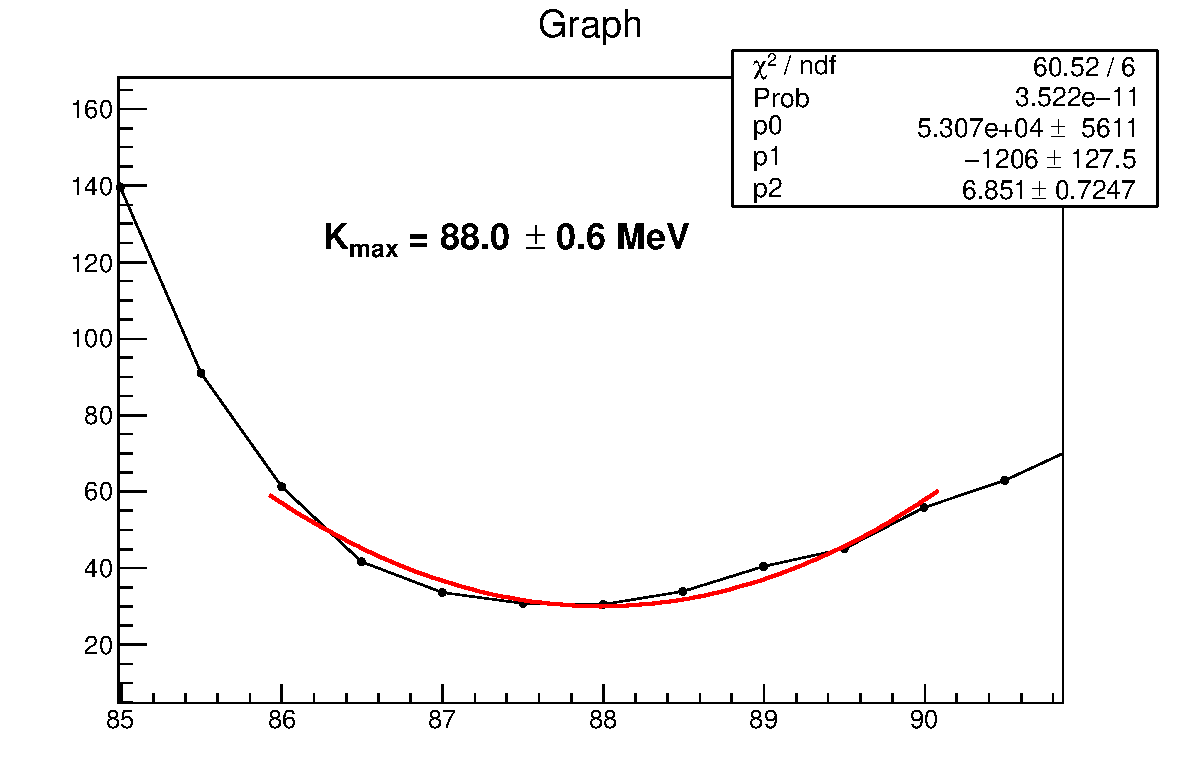
\includegraphics[width=1.0\textwidth]{figures/pdf/ana_step2_fit_kmax}
    }
  };
  % \node [text width=6cm, scale=0.8] at (4.5,6.4) {mu2e-18894 by Kevin Lynch and Jim Popp};
\end{tikzpicture}
\captionof{figure} {
  \label{fig:ana_step2_fit_kmax}
  $\bf k_m$ fit of the SINDRUM-II positron spectrum, energy losses are not
  taken into account
}
\vspace{0.1in}


Figure \ref{fig:ana_step2_ppos_best_fit} overlays the SINDRUM-II positron spectrum on
\Au{197}\ target with the closure approximation spectrum convoluted with the 
parameterized model of the SINDRUM-II detector response.

There are 14 events above 88 MeV in the data.

Looking at the data above 94 MeV, we can estimate the background due to radiative
pion capture (RPC) and cosmics to be of the order of one event.
Prediction of the closure approximation-based RMC model gives significantly less
than one event.

We therefore need to ask whether the closure approximation gives a reliable
description of the RMC positron spectrum near the end point. The closure approximation
doesn't take into account transitions to the exclusive low-lying states of the daughter
nucleus.

In case of the \Au{197} target, a transition \Au{197} --> $^{197}Pt$ to
the ground state of Pt nucleus is allowed. Given that the energy splitting between
an electron and a positron from the photon conversion is almost uniform,
the positron spectrum corresponding to such a transition, in a first approximation,
should be flat. 

probability of the order of $10^-3$, 

\vspace{0.1in}
\begin{tikzpicture}
  \node[anchor=south west,inner sep=0] at (0,0.) {
    % \node[shift={(0 cm,0.cm)},inner sep=0,rotate={90}] at (0,0) {}
    \makebox[\textwidth][c] {
      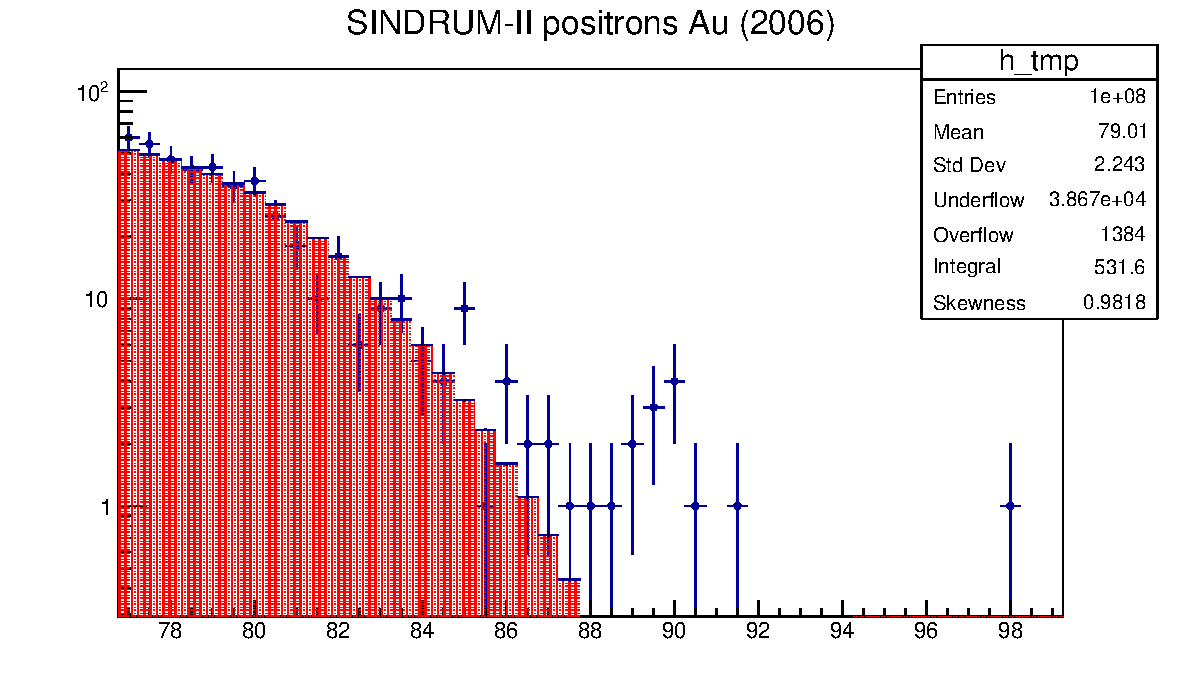
\includegraphics[width=1.0\textwidth]{figures/pdf/ana_step2_ppos_best_fit}
    }
  };
  % \node [text width=6cm, scale=0.8] at (4.5,6.4) {mu2e-18894 by Kevin Lynch and Jim Popp};
\end{tikzpicture}
\captionof{figure} {
  \label{fig:ana_step2_ppos_best_fit}
  best fit of the SINDRUM-II positron spectrum with closure approximation spectrum 
  convoluted with the parameterized model of the SINDRUM-II detector response
}
\vspace{0.1in}

%%%%%%%%%%%%%%%%%%%%%%%%%%%%%%%%%%%%%%%%%%%%%%%%%%%%%%%%%%%%%%%%%%%%%%%%%%%%%%
\subsection{Final states with the broken down  daughter nucleus}

As the daughter nucleus can break down, one could ask whether photons from
transitions
$$
\mu + \Au{197} \rightarrow \gamma + \nu + ^{197-k}Pt + k \rm neutrons
$$
or 
$$
\mu + \Au{197} \rightarrow \gamma + \nu + ^{197-k}A_{Z=79-k} + k \rm protons
$$

could have a higher spectrum end point. Figure ~\ref{fig:pt197_dmass} shows the
mass differences for the two different schenarios, 
  
\vspace{0.1in}
\begin{tikzpicture}
  \node[anchor=south west,inner sep=0] at (-2.0,0.0) {
    % \node[shift={(0 cm,0.cm)},inner sep=0,rotate={90}] at (0,0) {}
    % \makebox[\textwidth][c] {
      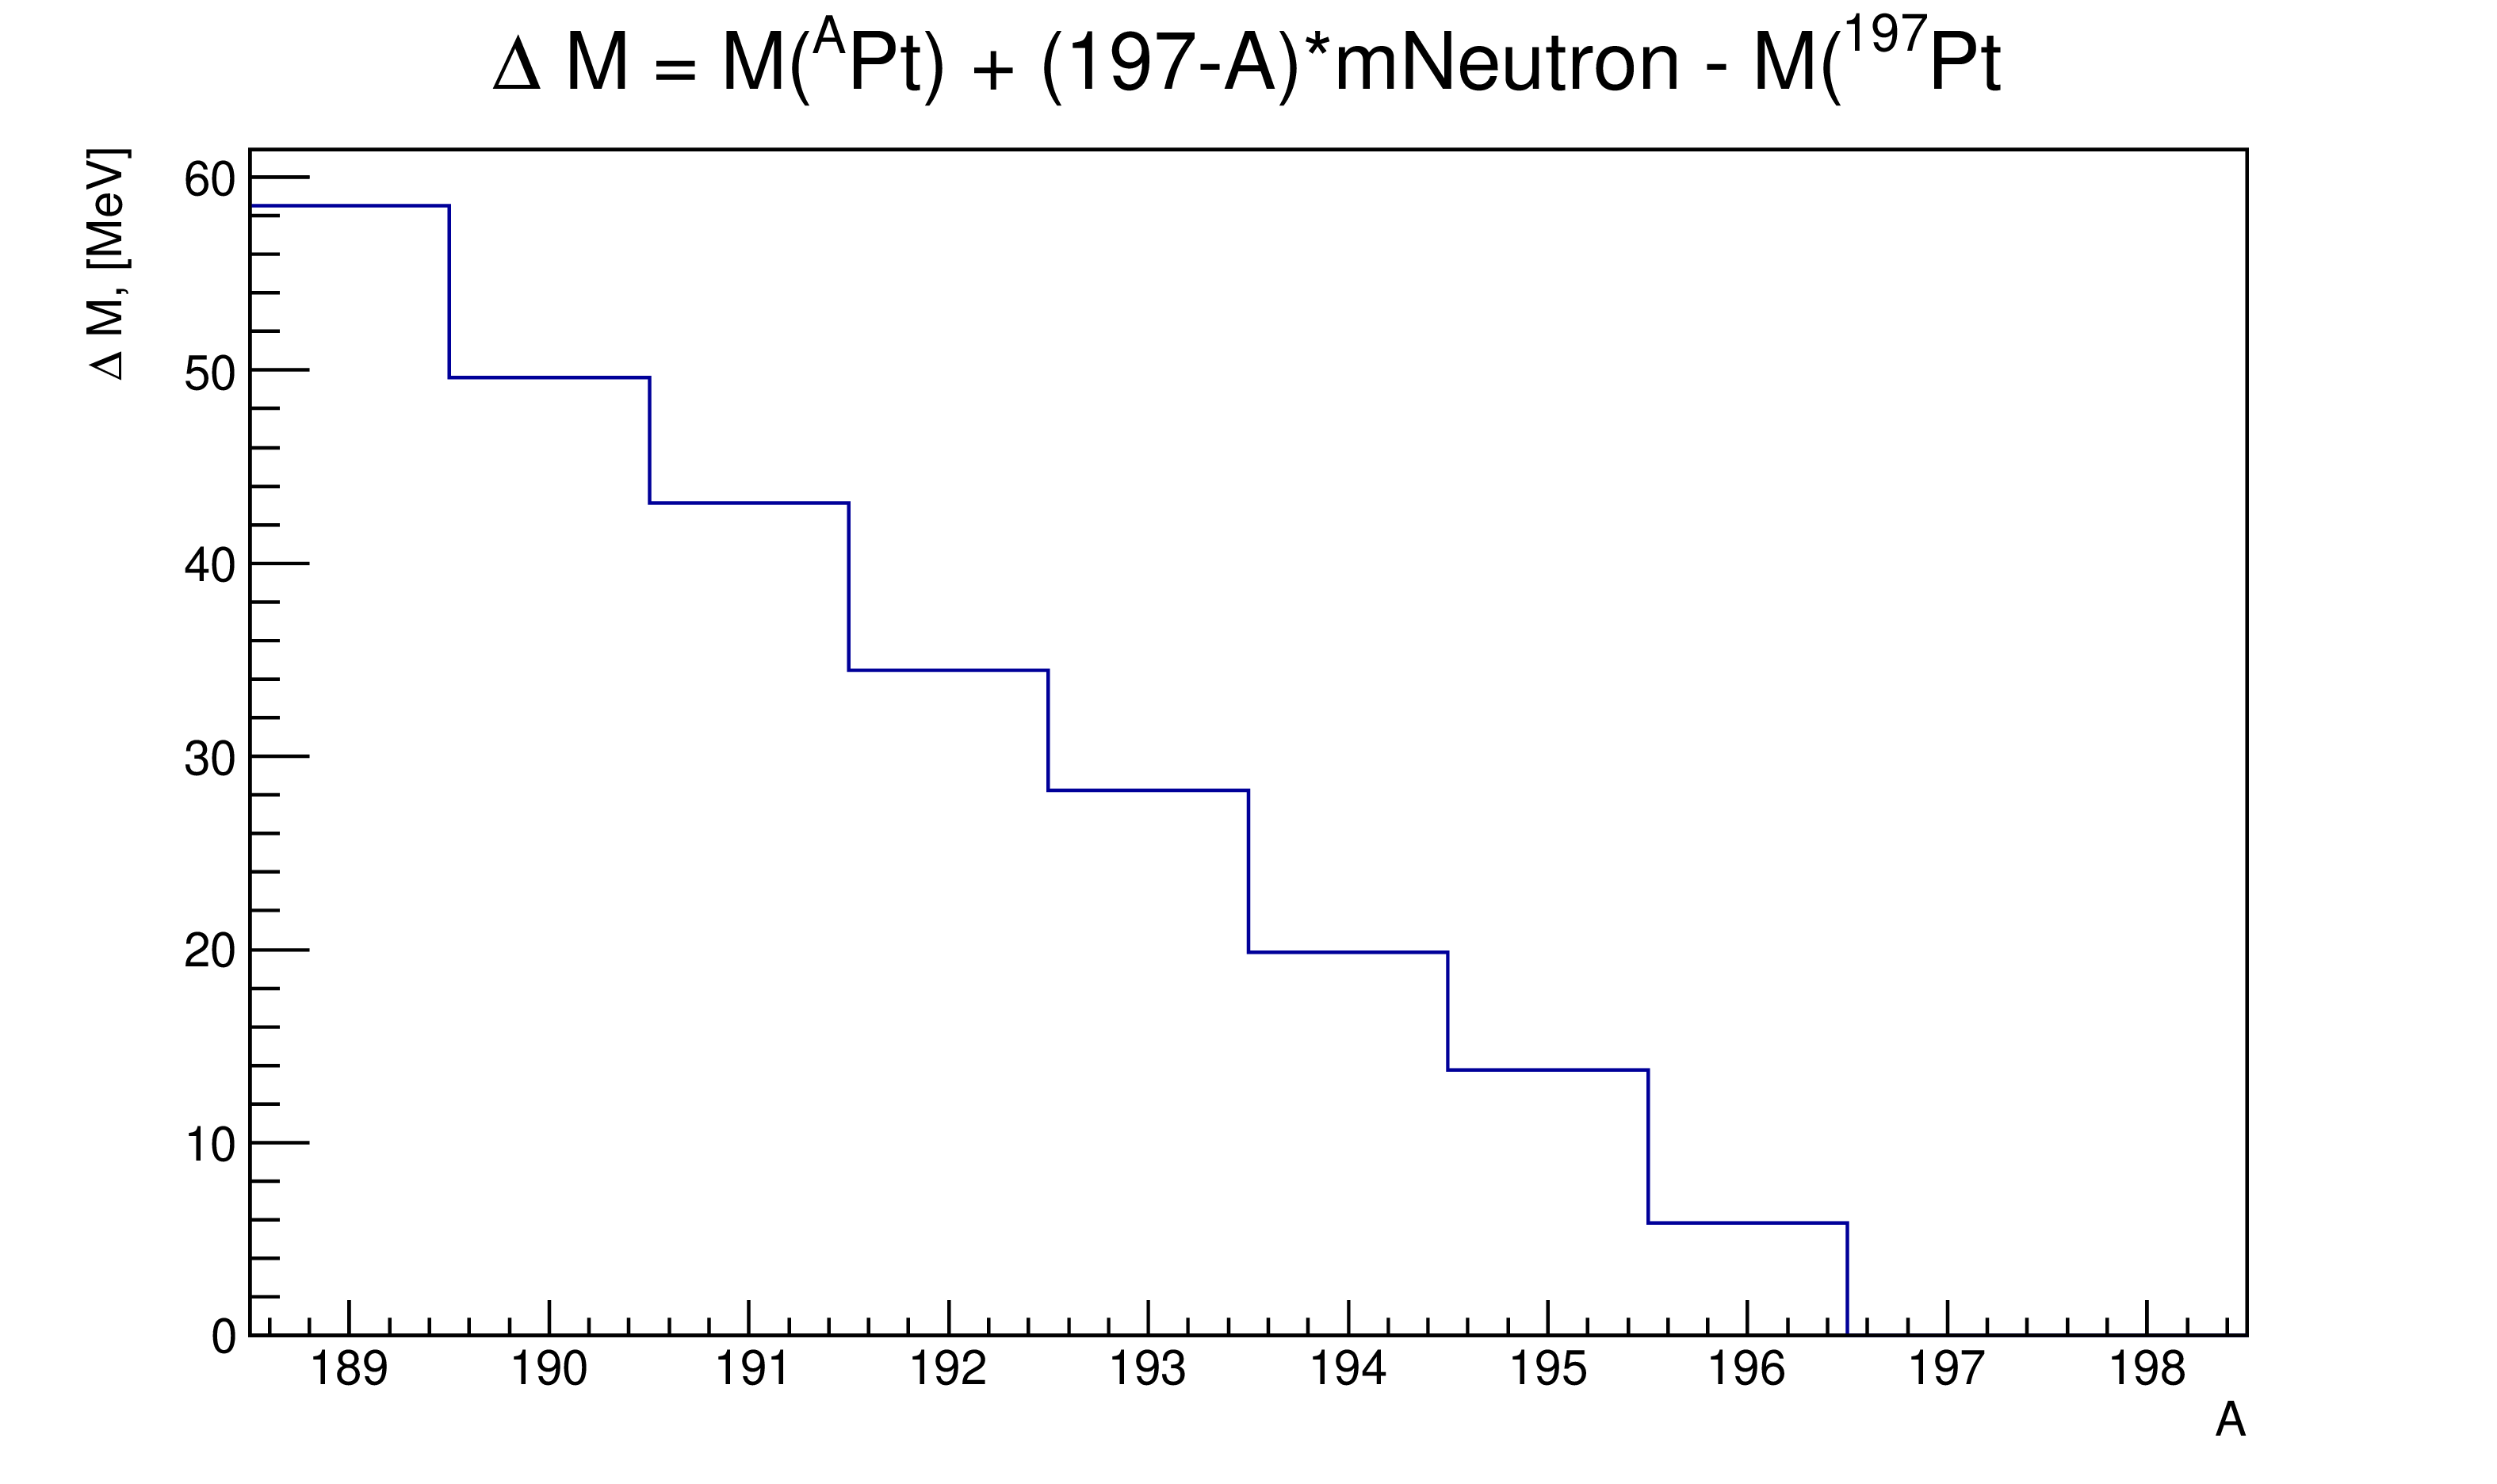
\includegraphics[width=0.6\textwidth]{figures/png/pt197_dmass}
    % }
  };
  \node[anchor=south west,inner sep=0] at (6.0,0.0) {
    % \node[shift={(0 cm,0.cm)},inner sep=0,rotate={90}] at (0,0) {}
    % \makebox[\textwidth][c] {
      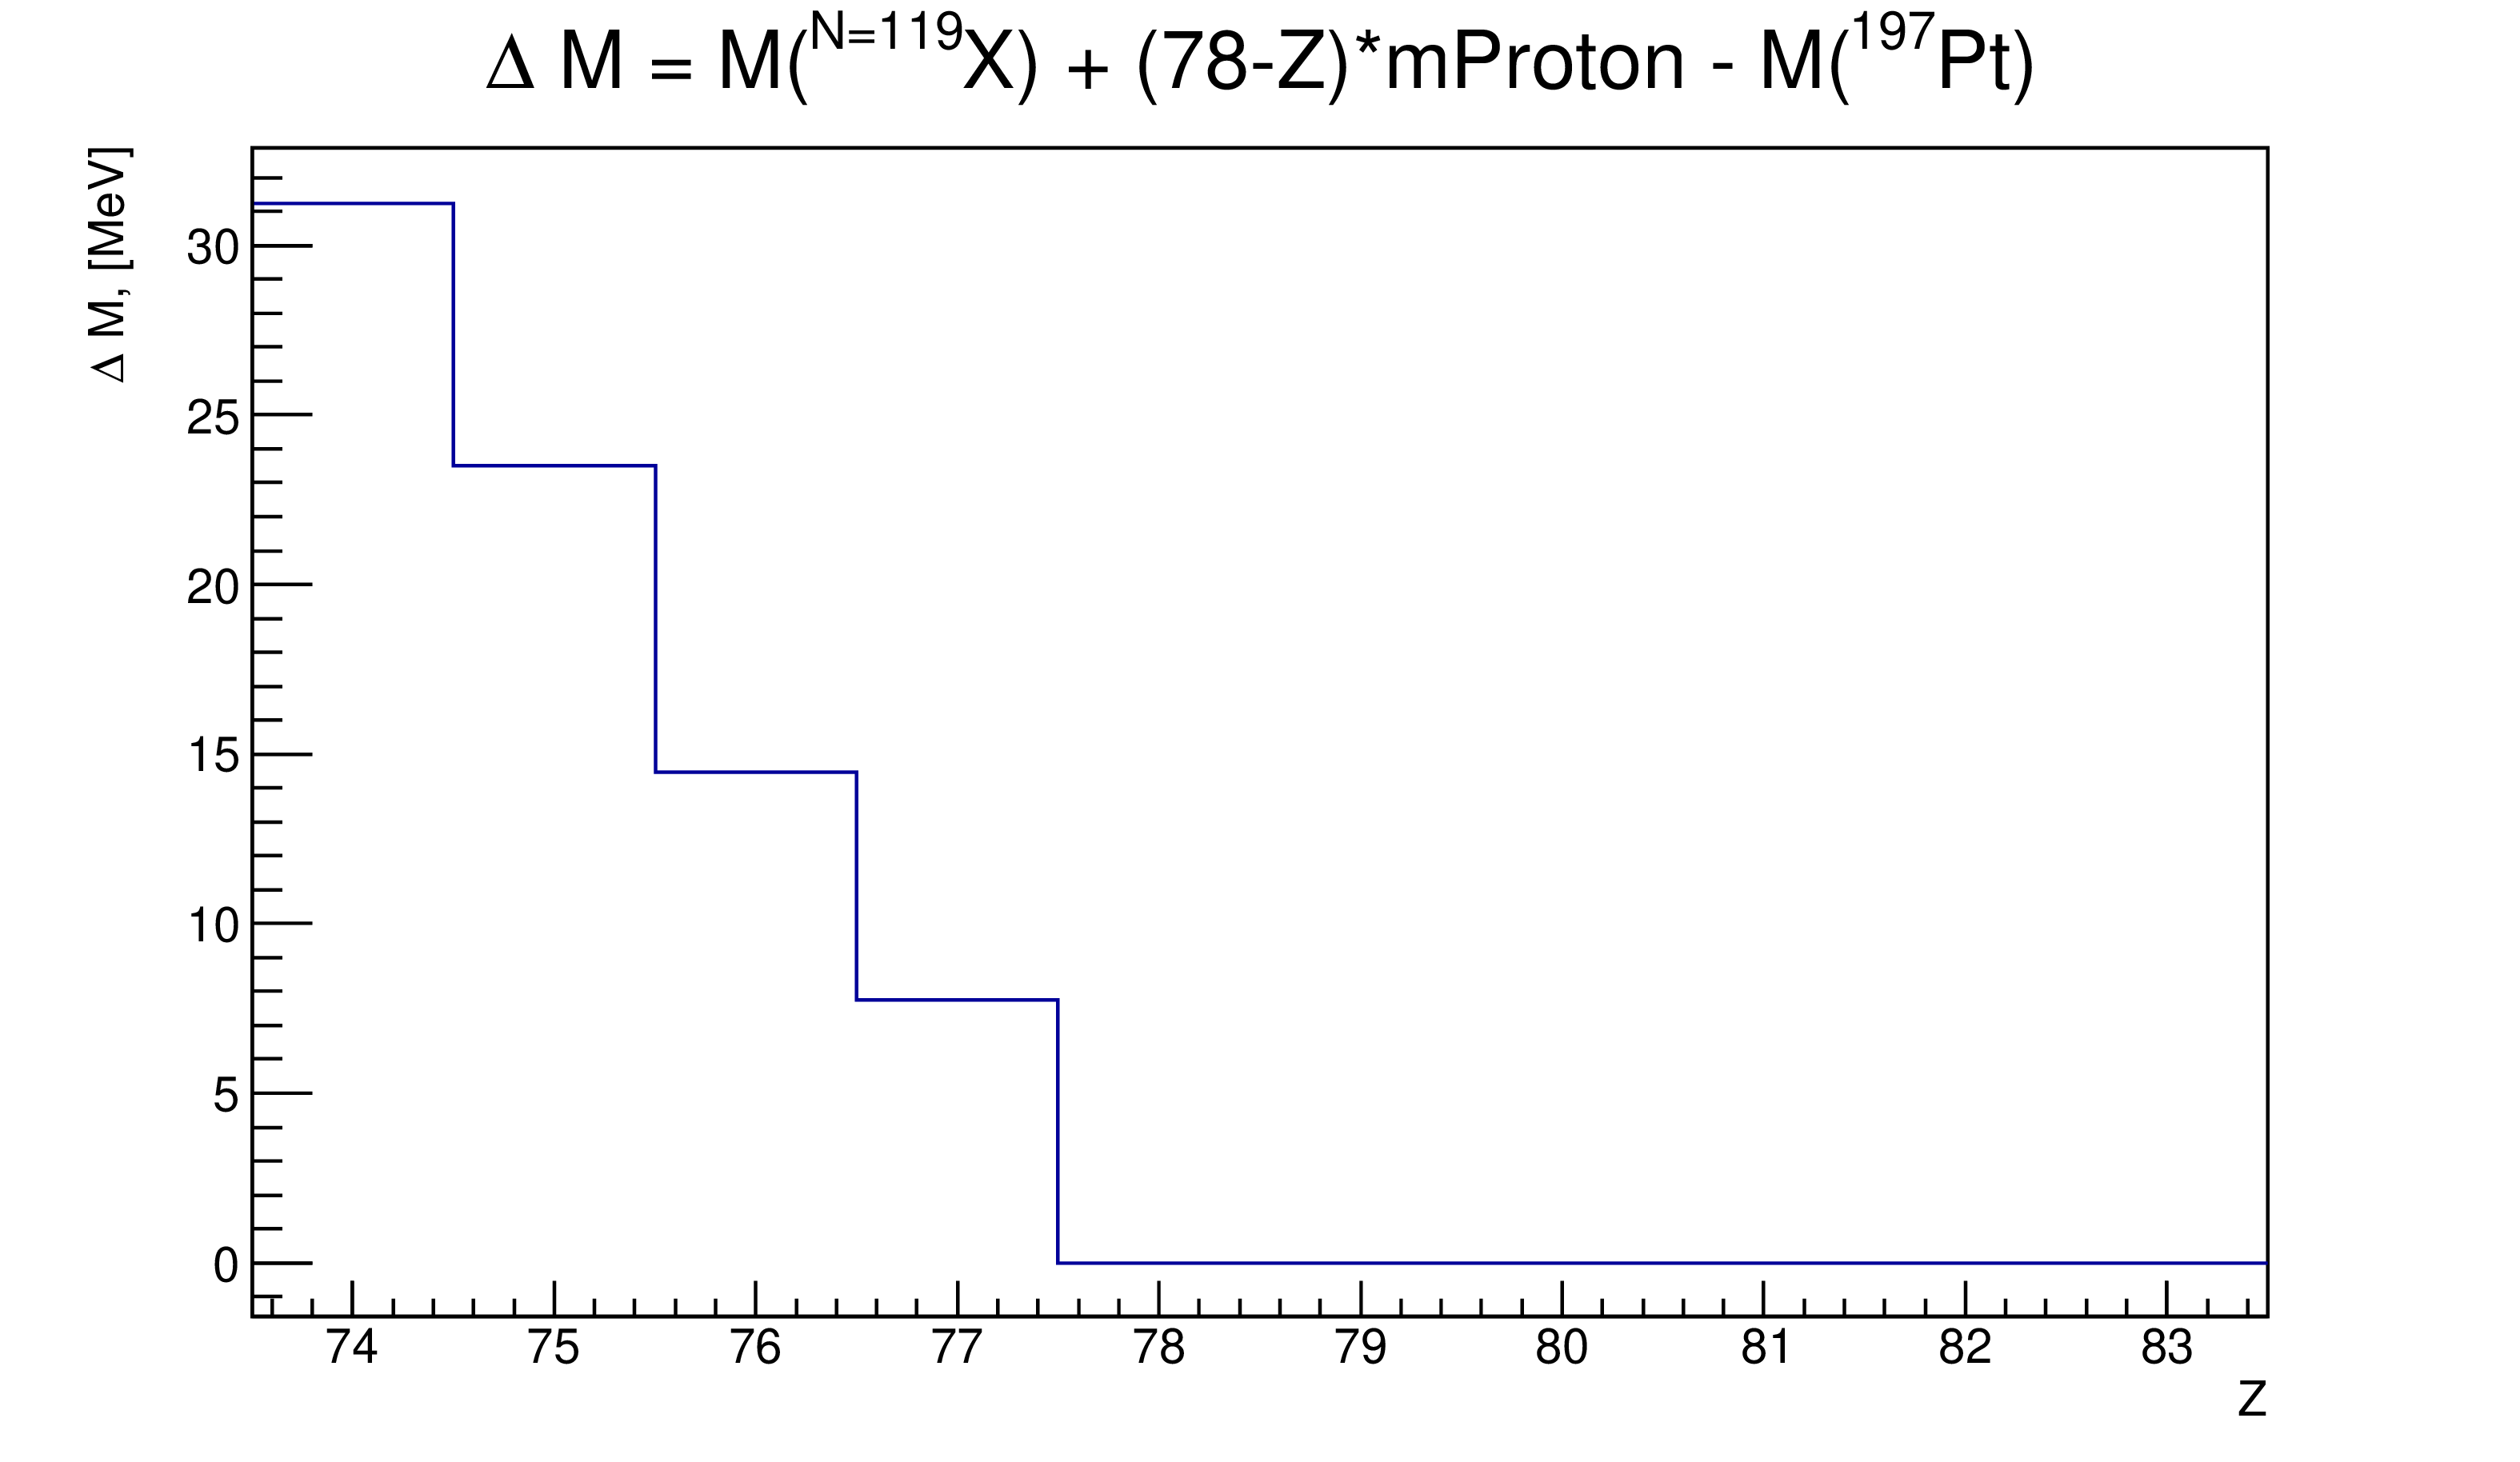
\includegraphics[width=0.6\textwidth]{figures/png/pt197_dmass_n}
    % }
  };
  % \node [text width=6cm, scale=0.8] at (4.5,6.4) {mu2e-18894 by Kevin Lynch and Jim Popp};
\end{tikzpicture}
\captionof{figure} {
  \label{fig:pt197_dmass}
  Mass differences between the final state with the broken down daughter nucleus
  and $^{197} Pt$ for different breakdown scenarios.
  The final state with ``unbroken'' $^{197} Pt$ always has the lowest mass and,
  therefore, the highest photon spectrum endpoint
}
\vspace{0.1in}

%%% Local Variables:
%%% mode: latex
%%% TeX-master: t
%%% End:
